% The first part of a .tex file is to include packages and define environment, you don't have to change anything but you are welcome to do that.
%%%%%%%%%%%%%%%%%%%%%%%%%%%%%%%%%%%%%%%%%%%%%%%%%%%%%%%%%%%%%%%%%%%%%%
\documentclass[letter,11pt]{article}

\usepackage{amsmath, amsthm,natbib}
\usepackage{amssymb}
\usepackage{graphicx}
\usepackage{subfig}
\usepackage{amsfonts}
\usepackage{rotating}
\usepackage[colorlinks, citecolor=blue, urlcolor=blue, pdfborder={0 0 1}, citebordercolor={1 1 1}]{hyperref}
\usepackage{hyperref}
\usepackage{algorithm}
\usepackage{algpseudocode}
\usepackage{listings}
\usepackage[most]{tcolorbox}
\usepackage{inconsolata}
\usepackage{minted}
\algrenewcommand{\Return}{\State\algorithmicreturn~}

\newtheorem{theorem}{Theorem}
% You can define anything you like to follow the same pattern as theorem.
\newtheorem{claim}[theorem]{Claim}
\newtheorem{lemma}[theorem]{Lemma}
\newtheorem{conjecture}[theorem]{Conjecture}
\newtheorem{corollary}[theorem]{Corollary}
\newtheorem{definition}[theorem]{Definition}

\renewcommand{\baselinestretch}{1.3}
\setlength{\textwidth}{18cm}
\setlength{\oddsidemargin}{-10mm}
\setlength{\evensidemargin}{-20mm}

% Here is where the real content starts.
%%%%%%%%%%%%%%%%%%%%%%%%%%%%%%%%%%%%%%%%%%%%%%%%%%%%%%%%%%%%%%%%%%%%%%%%
\title{Assignment 6}

\author{Naga Nithin Manne \& Dipti Sengupta\\ MPCS 51300, University of Chicago}

\date{} % The default is today

% Start the document environment for whatever you want to display in the pdf file.
\begin{document}
\maketitle % Insert the title, author and date

\section*{Compile Time vs. Speed}

We are going to investigate the following three optimization techniques on a few simple test programs
\begin{itemize}
  \item Inlining
  \item InstCombine
  \item All Available Optimizations
\end{itemize}

\textbf{Note:} The resolution of the times are approximately 1 ms. It was not possible to get higher precision in Python without linking to Windows APIs.

\subsection*{Inlining}

\subsubsection*{Test Program}

\begin{minted}{Perl}
extern int arg(int);

def int add(int $x, int $y) { return $x + $y; }

def int run() {
    int $n = arg(0);
    int $i = 0;
    int $j = 0;
    int $s = 0;
    while ($i < $n) {
        $j = 0;
        while ($j < $n) {
            $s = add($s, $i);
            $j = $j + 1;
        }
        $i = $i + 1;
    }
}
\end{minted}

Function Inlining can be used to improve the performance of the call to $add$, which is done $n^2$ times in the test program. From the below graph, we can see that this optimization is very quick and offers performance improvements for even small values of $n$.\\
\textbf{Time taken for Optimization:} 0.0009965896606445312

\begin{figure}[H]
	\centering
	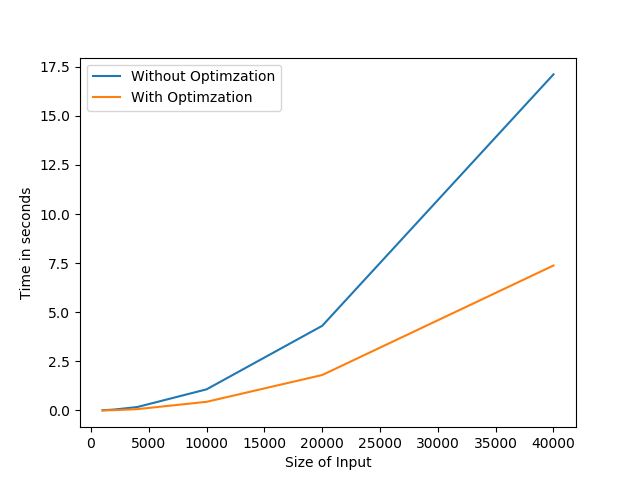
\includegraphics[width=10cm]{timing/1.png}
	\caption{Inlining}
	\label{fig:inlining}
\end{figure}


\subsection*{InstCombine}

\subsubsection*{Test Program}

\begin{minted}{Perl}
extern int arg(int);

def int run() {
    int $n = arg(0);
    int $i = 0;
    int $j = 0;
    int $s = 0;
    while ($i < $n) {
        $j = 0;
        while ($j < $n) {
            $s = $s + 1;
            $s = $s + 1;
            $s = $s + 1;
            $s = $s + 1;
            $s = $s + 1;
            $s = $s + 1;
            $s = $s + 1;
            $s = $s + 1;
            $s = $s + 1;
            $s = $s + 1;
            $j = $j + 1;
        }
        $i = $i + 1;
    }
}
\end{minted}

InstCombine can be used to combine multiple instructions like the additions above into a single instruction which can reduce the clock cycles needed to execute the program. Here, the cost of optimization is just high enough that its is more efficient to not perform optimization for smaller input sizes.\\
\textbf{Time taken for Optimization:} 0.0019943714141845703
\begin{figure}[H]
	\centering
	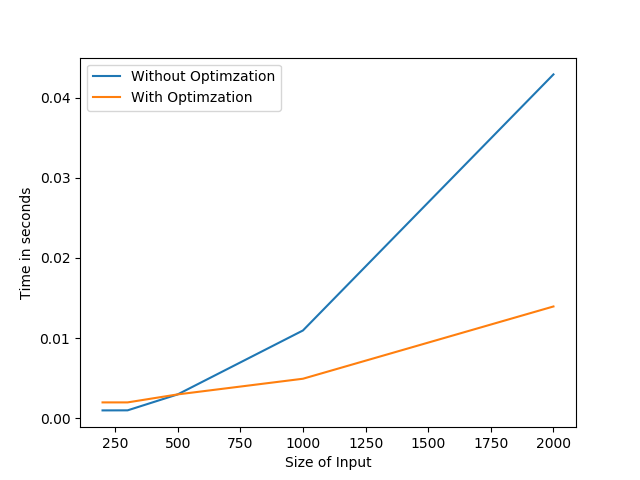
\includegraphics[width=10cm]{timing/2.png}
	\caption{InstCombine}
	\label{fig:instcombine}
\end{figure}

\subsection*{All Available Optimizations}

\subsubsection*{Test Program}

\begin{minted}{Perl}
extern int arg(int);

def int fib(int $n) {
    if ($n == 0 || $n == 1) return $n;
    else return fib($n - 1) + fib($n - 2);
}

def int run() {
    int $n = arg(0);
    print fib($n);
}
\end{minted}

In this test code, the fibonacci sequence cannot be optimized since the recursion algorithm has no possible optimizations. So in this scenario, the performance improvement due to optimization is minor as from the graph below.\\
\textbf{Time taken for Optimization:} 0.001962900161743164

\begin{figure}[H]
	\centering
	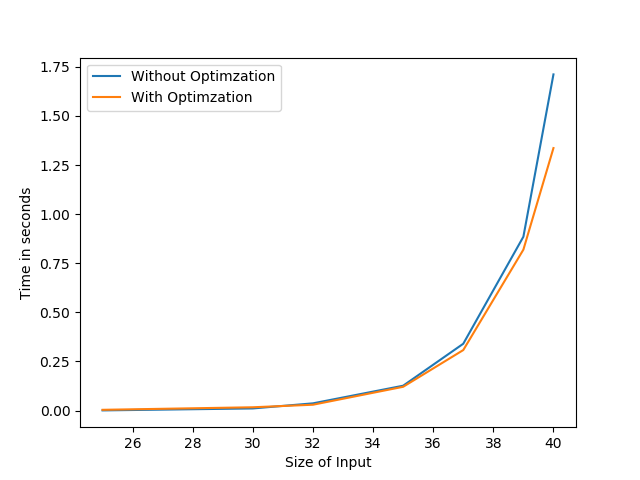
\includegraphics[width=10cm]{timing/3.png}
	\caption{AllOptimzations}
	\label{fig:all}
\end{figure}

% Don't forget to end the document environment in the end.
\end{document}